%!TEX root = main.tex

\section{Results}\label{Results}


\subsection{Hypothesis~\ref{Hip:AndOverOr}}\label{Results:AndOverOr}
We asked whether the conjunction-disjunction bias (which is known to affect learning times in the case of a single explanation \cite{bourne1970knowing}) also determines which features are used to describe a concept when two alternative explanations are consistent with the observed universe. In the first trial, the observed examples were consistent with $p_1 \vee p_2$ and with $p_3 \wedge p_4$. As explained in \S\ref{Subsec:ExperimentFlow}, in the generalization stage we can determine if participants explained the concept using $\{p_1,p_2\}$ or $\{p_3,p_4\}$. We found that 77 of the 100 participants attended to $\{p_3,p_4\}$, which corresponds to an explanation that uses a conjunction. 11 participants attended to $\{p_1,p_2\}$ (corresponding to the use of a disjunction for the explanation), and 12 participants selected examples in the generalization stage inconsistent with both $p_3 \wedge p_4$ and $p_1 \vee p_2$. To test the significance of this result, we performed a permutation test. Under the null hypothesis that participants randomly choose between explaining the concept using features $\{p_1,p_2\}$ and explaining it using $\{p_3,p_4\}$, the probability that 77 of the 100 participants attend to $\{p_3,p_4\}$ is $P<10^{-12}$. Thus we conclude that the observed difference is significant. 

Note that it is in principle possible that the participant learned the concept with a focus on negative examples ({\sf B}'s in Figure~\ref{fig:trials}) instead of on positive examples ({\sf A}'s in Figure~\ref{fig:trials}) (i.e. finding a correct explanation for the negative examples and then negating that rule to obtain an explanation for the positive examples). 

As we mention in \S\ref{Experiment_design}, we induced a bias to understand the concept in the appropriate way by first presenting the positive examples in the learning phase and by asking them to click on the positive ones in the training phase. We note, however, that 9 participants gave verbal explanations consistent with focusing on the negative examples. In this particular trial, a reverse interpretation is problematic since the negation of a conjunction corresponds to a disjunction, and the negation of the disjunction to a conjunction (i.e.\ $p\land q$ is logically equivalent to $\lnot(\lnot p\lor \lnot q)$). Thus, a more comprehensive analysis should take into account participants' verbal explanations in this trial. However, even considering the worst-case scenario in which these 9 participants were originally regarded as part of the `conjunction' group and they are now considered part of the `disjunction' group, the conjunction-disjunction bias is still significant ($P<10^{-7}$). We therefore conclude that, in this framework where multiple explanations are possible depending on the attended features, there is a bias favoring conjunctive explanations over disjunctive explanations. 

\subsection{Hypothesis \ref{Hip:FeatureBiasStickiness}}\label{Results:FeatureBiasStickiness}   
Most participants understood the concept in Trial 6 using the same features $\{p_7,p_8\}$ used to describe the concept in Trial~5, even when the logical structure of the rule was exactly the same independently of attending to $\{p_7,p_8\}$ or to $\{p_3,p_4\}$\footnote{As expected by our experiment design, 94 of the 100 participants understood the concept in Trial 5 using features $\{p_7,p_8\}$ (6 selected features with no clear rationale). Using features $\{p_7,p_8\}$ is indeed the only plausible way to learn the concept, given the high complexity of the alternative MDL15 formula. }. To show this, we study participants' choices in the generalization stage of Trial 6 (see Figure~\ref{fig:results1}). 

Suppose that a participant is thinking of the rule $\lnot p_7 \land \lnot p_8$, thus they are only attending to features $\{p_7,p_8\}$ while ignoring the features $\{p_3,p_4\}$. Since $\{p_3,p_4\}$ are being ignored, the participant should mark those elements in which $\{p_7,p_8\}$ agrees with the rule $\lnot p_7 \land \lnot p_8$, irrespective of the values of $\{p_3,p_4\}$. That is, the participant should mark the elements with $\{p_3,p_4,p_7,p_8\}$ equal to $(0,0,\textbf{0,0})$, $(1,0,\textbf{0},\textbf{0})$, $(0,1,\textbf{0},\textbf{0})$ and $(1,1,\textbf{0},\textbf{0})$. These elements have $\{p_7,p_8\}$ equal to $(0,0)$ and `anything' for $\{p_3,p_4\}$. On the other hand, if the participant is thinking of the rule $p_3 \land \lnot p_7 \land \lnot p_8$, then she is attending to $\{p_3,p_7,p_8\}$, and she should mark $(\textbf{1},0,\textbf{0},\textbf{0})$ and $(\textbf{1},1,\textbf{0},\textbf{0})$. 

In general, by studying which of the 7 examples shown in Figure~\ref{fig:results1} (left) the participant selects in the generalization phase, we can deduce which features they were attending to (Figure~\ref{fig:results1}, right). For example, all participants should mark the example with $\{p_3,p_4,p_7,p_8\}$ equal to $(1,1,0,0)$, since it is consistent with all the logical rules irrespective of which features are used. 

Indeed, as shown in Figure~\ref{fig:results1} (left), all participants selected this example. Although in practice the participant can select any of the 7 examples in the generalization stage, we found that all but five participants respected the rules of coherence illustrated in the previous paragraph. These 5 participants were `one example away' of respecting the rule, however, we leave them out of the feature stickiness analysis, but including them does not change our conclusions. We also excluded 6 participants that selected elements with no clear rationale in the previous trial, since they may not have used features $\{p_7,p_8\}$. However, including these participants (and assuming they did use $\{p_7,p_8\}$ in the previous trial) does not significantly change the results. In total, these two exclusions leaves 89 participants for this analysis. The grey lines in Figure~\ref{fig:results1} (left) show simulations of agents that randomly select one of the seven possible subsets of features, and then proceed to select the examples consistent with the logical rule using that features. Participants responses (black line) were biased towards explanations using $\{p_7,p_8\}$, as predicted by the feature-stickiness bias. This can also be seen in  Figure~\ref{fig:results1} (right), after inferring which features participants used to build the rule for the concept. In addition to being biased towards $\{p_7,p_8\}$, several participants explained the concept using all available features $\{p_3,p_4,p_7,p_8\}$. This shows that, in addition to the feature stickiness bias, when the number of features is relatively small, participants were also biased to describe the concept using all available features.

To quantify the feature stickiness bias, we assign a score to each participant according to the attended features in Trial 6 (deduced from the marked examples). The scores for the subsets $\{p_7,p_8\}$, $\{p_3,p_7,p_8\}$, $\{p_4,p_7,p_8\}$, $\{p_3,p_4,p_7,p_8\}$, $\{p_3,p_4,p_7\}$, $\{p_3,p_4,p_8\}$ and $\{p_3,p_4\}$ are 1, 2/3, 2/3, 1/2, 1/3, 1/3 and 0 respectively\footnote{Part (d) of the Analysis Plan section in our preregistration had a mistake in the use of features names: the learnable concept corresponding to the fifth trial uses $p_7$ and $p_8$, not $p_3$ and $p_4$ as erroneously written in that part; compare with the section on Study design, which matches Table~\ref{trial_table}.}. The average score for the 89 participants was 0.68 ($P<10^{-6}$ in a permutation test with the null hypothesis of randomly attending to one of the seven subsets of features, which correspond to the grey lines in Figure~\ref{fig:results1}), indicating a significant effect of the feature stickness bias. Although the feature stickiness bias was significant for both groups independently (Group X: average score 0.62, $P<10^{-5}$;  Group Y: average score 0.74, $P<10^{-6}$), we found that feature stickiness was higher in Group Y (two-sample t-test comparing the scores of the two groups shows $t=2.35$,  $P<0.05$). The only difference between the groups is that Group Y had already (artificially) experienced feature stickiness between the previous Trials 3 and 4, so they have already identified it as an useful bias for the task. This suggests that the entire concept-learning sequence can be important when studying learning biases. %even concepts learnt several trials in the past.

\begin{figure}
\begin{center}
	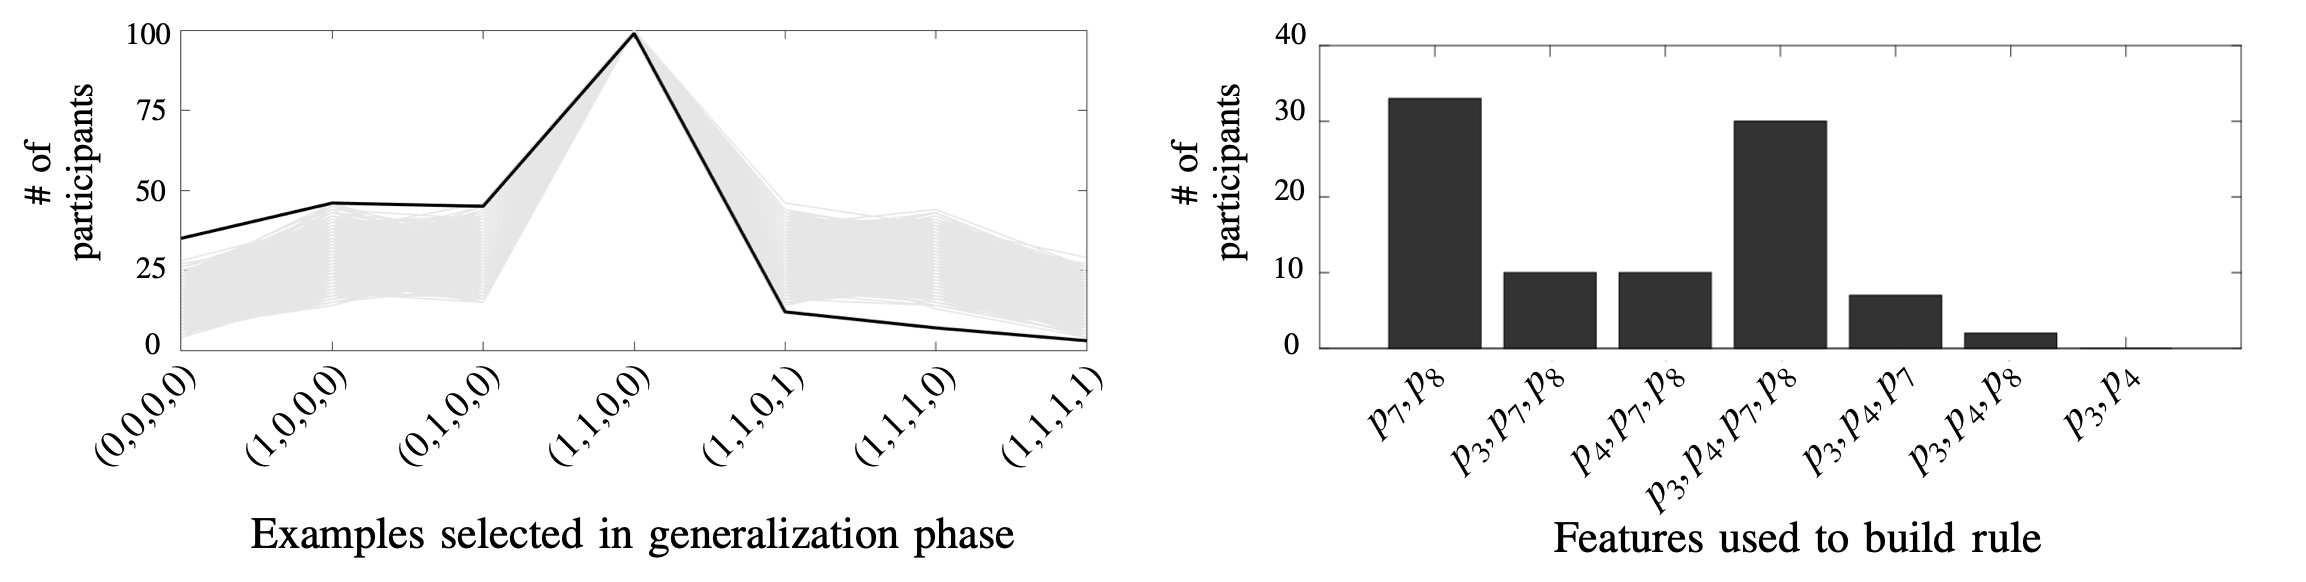
\includegraphics[scale=.37]{Images/results_1.png}
\end{center}\caption{\textbf{(Left)} Number of participants (100 participants total) that, in the generalization stage of Trial 6, selected an element (possibly among others; the numbers add up to more than 100) with the elements written on the x-axis, indicating the values of the features $\{p_3,p_4,p_7,p_8\}$ respectively. As multiple choices were possible, the sum for all choices adds up to a value greater than 100. In grey we show 100,000 simulations in which 100 agents randomly attend to one of the seven subset of features (see text). \textbf{(Right)} From the selected objects in the generalization phase we can infer which features participants used to build the rule for the concept (89 valid participants, see main text).}
\label{fig:results1}
\end{figure}

 
 \begin{figure}
\begin{center}
	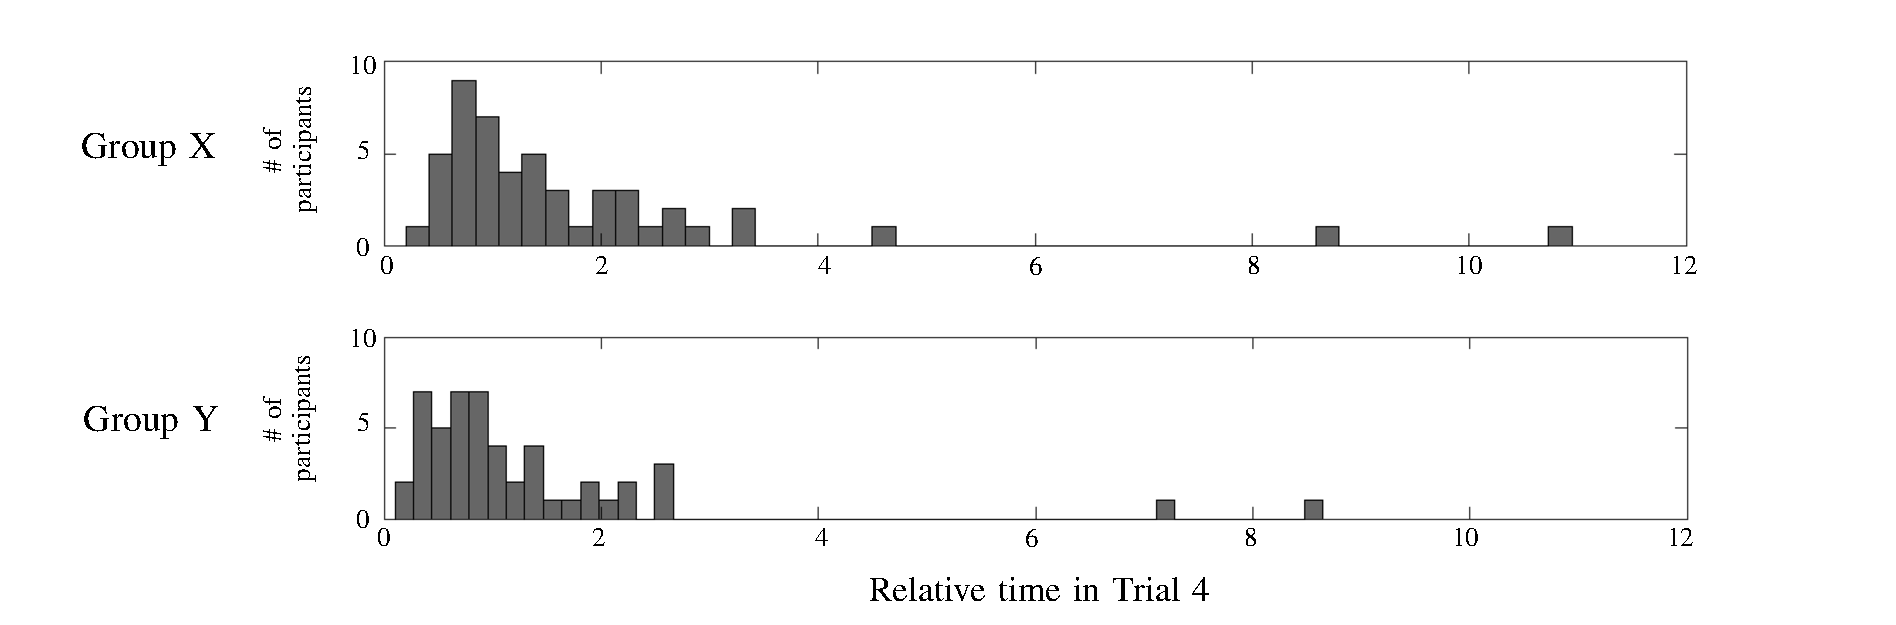
\includegraphics[scale=.5]{Images/results_2.pdf}
\end{center}\caption{Relative time spent in Trial 4 by participants from the two groups, normalized by the time spent in Trial 5.}
\label{fig:results2}
\end{figure}



\subsection{Hypothesis \ref{Hip:FeatureBiasTimeAdvantage}}\label{Results:FeatureBiasTimeAdvantage} 
This hypothesis regarded the behavioral advantage of the feature stickiness effect, which we tested by comparing learning \emph{times} in Trial 4 for participants of Groups X versus Y (see Figure~\ref{fig:results2}).
If the feature stickiness bias represents a behavioral advantage, Group Y should learn concept $C^4_1$ \emph{faster} than Group X. To avoid confounds due to inter-individual differences in absolute learning time, for this analysis we normalize individual learning times with the time spent in Trial 5, which uses different features than the previous concepts and should not be affected by any obvious inter-trial relation with previous concepts\footnote{Indeed, Trial 5 was pre-registered as a `normalizer' trial.}. Thus we compare between the two groups (X and Y) the time spent in Trial 4 divided the time expended in Trial 5. This gives one number for each participant, and we compare the lists of numbers of the two groups using a two-sample t-test.  The differences in the learning times between the groups are not significant if we analyze the data of all participants as shown in Figure~\ref{fig:results2} (two-sample t-test shows $t_{98}=1.26 \ $,  $P=0.2$; Cohen's $d=0.25$), but they are significant if we rule out from this analysis 5 outliers that spent more than 5 times in concept 4 than 5, or in concept 5 than 4 ($t_{98}=2.18 \ $,  $P<0.05$, Cohen's $d=0.42$)\footnote{The ANOVA proposed in the pre-registration also did not reveal significant differences in learning times. For simplicity in the analysis of the outliers, we replaced here the ANOVA for a simple t-test between the normalized learning times of the two groups.}.



\subsection{Hypothesis \ref{Hip:StickinessFeatureOperator}} \label{Results:StickinessFeatureOperator} 
The idea of this hypothesis is to test if participants prefer sticking to operators or sticking to features form one trial to the next. In this work we did not find conclusive evidence regarding this hypothesis. We suspect that the cause was an experimental setup that underestimated the strength of the bias favoring the $\AND$ operator over the $\OR$ operator. We found that 77 of the 100 participants explained Trial 1 using $\AND$, 11 explained it using $\OR$ and 12 selected elements in the generalization phase with no clear rationale. Of the 77 that used $\AND$, 64 also used $\AND$ in Trial 2, thus changing features but maintaining operator; and 7 of them used $\OR$, changing operator but maintaining features (the other 6 selected elements with no clear rationale). Of the 11 that used $\OR$, 10 used $\AND$ in Trial 2, changing operator but maintaining features; and 1 of them used $\OR$ in the second trial. We realize, however, that a change from using $\OR$ in the first concept to $\AND$ in the second one could not only be due to the effect of feature stickiness, but also simply to the stronger preference for $\AND$. Thus without a precise quantitative knowledge of the prior preference of $\AND$ over $\OR$, we cannot conclude about the effect of operator stickiness vs.\ feature stickiness. A future experiment could probe the existence of operator stickiness by having longer consecutive periods where feature reuse is not a useful bias and where only one logical operator remains useful for explaining a concept, before finally presenting a concept that can be explained via two different rules, each using different operators. Thus we leave for future work the task of studying the interaction between the feature stickiness bias and the precise structure of the logical rules being learnt. 



\subsection{MDL bias} \label{Resultados:MDLbias} 

The MDL-bias hypothesis posits that concept-learning difficulty increases with its MDL \cite{feldman2000minimization}. %\sergio{\cite{feldman2003simplicity}?}
In addition to their other roles, Trials 3 (group X and Y), 4, and 5 served to test this hypothesis in the new framework of multiple consistent explanations. In these trials, there were two possible explanations that were consistent with the shown data, one of much higher MDL than the other (15 vs.\ 3). For example, in the Group X of Trial~3, the short explanation was $p_1 \land p_2$, while the longer one was $((p_3 \lor (p_4 \lor p_5))\land(\lnot p_3 \lor ((p_4 \lor \lnot p_5)\land (p_5 \lor \lnot p_4))))$; the longer rule in other trials was always a substitution of features applied to this one (in order to keep the features disjoint between the two explanations). For these 3 trials, the responses of the $100$ participants add to a total of $300$ responses. From this total, $18$ responses in the generalization phase did not choose objects consistent with any of the two explanations; $2$ responses were consistent with the MDL~15 rule; and $280$ responses were consistent with the MDL~3 rule. While this was expected by the experimental design (since we included a MDL~15 rule in those trials where we wanted to bias the participants into finding the other rule), we conclude that the MDL-bias hypothesis holds in this framework of multiple consistent explanations. Future work could explore in greater detail the relative difficulty of rules with slightly different MDL in this framework.
